%%%%%%%%%%%%%%%%%%%%%%%%%%%%%%%%%%%%%%%%%%%%%%%%%%%%%%%%%%%%%%%%%%%%%%%%%%%%%%%%
%
% Template license:
% CC BY-NC-SA 3.0 (http://creativecommons.org/licenses/by-nc-sa/3.0/)
%
%%%%%%%%%%%%%%%%%%%%%%%%%%%%%%%%%%%%%%%%%%%%%%%%%%%%%%%%%%%%%%%%%%%%%%%%%%%%%%%%

%----------------------------------------------------------------------------------------
%	PACKAGES AND OTHER DOCUMENT CONFIGURATIONS
%----------------------------------------------------------------------------------------

\documentclass[
11pt, % The default document font size, options: 10pt, 11pt, 12pt
%oneside, % Two side (alternating margins) for binding by default, uncomment to switch to one side
%chapterinoneline,% Have the chapter title next to the number in one single line
spanish,
singlespacing, % Single line spacing, alternatives: onehalfspacing or doublespacing
%draft, % Uncomment to enable draft mode (no pictures, no links, overfull hboxes indicated)
%nolistspacing, % If the document is onehalfspacing or doublespacing, uncomment this to set spacing in lists to single
%liststotoc, % Uncomment to add the list of figures/tables/etc to the table of contents
%toctotoc, % Uncomment to add the main table of contents to the table of contents
parskip, % Uncomment to add space between paragraphs
%codirector, % Uncomment to add a codirector to the title page
headsepline, % Uncomment to get a line under the header
]{MastersDoctoralThesis} % The class file specifying the document structure



%----------------------------------------------------------------------------------------
%	INFORMACIÓN DE LA MEMORIA
%----------------------------------------------------------------------------------------

\thesistitle{Desarrollo de un \emph{mesh protocol stack} para HRD-Radio LoRa} % El títulos de la memoria, se usa en la carátula y se puede usar el cualquier lugar del documento con el comando \ttitle

% Nombre del posgrado, se usa en la carátula y se puede usar el cualquier lugar del documento con el comando \degreename
%\posgrado{Carrera de Especialización en Sistemas Embebidos} 
\posgrado{Carrera de Especialización en Internet de las Cosas} 
%\posgrado{Carrera de Especialización en Intelegencia Artificial}
%\posgrado{Maestría en Sistemas Embebidos} 
%\posgrado{Maestría en Internet de las cosas}

\author{Ing. Ricardo Losada} % Tu nombre, se usa en la carátula y se puede usar el cualquier lugar del documento con el comando \authorname

\director{Téc. Mariano Hunkeler (RF Industrial)} % El nombre del director, se usa en la carátula y se puede usar el cualquier lugar del documento con el comando \dirname
\codirector{Nombre del codirector (pertenencia)} % El nombre del codirector si lo hubiera, se usa en la carátula y se puede usar el cualquier lugar del documento con el comando \codirname.  Para activar este campo se debe descomentar la opción "codirector" en el comando \documentclass, línea 23.

\juradoUNO{Nombre del jurado 1 (pertenencia)} % Nombre y pertenencia del un jurado se usa en la carátula y se puede usar el cualquier lugar del documento con el comando \jur1name
\juradoDOS{Nombre del jurado 2 (pertenencia)} % Nombre y pertenencia del un jurado se usa en la carátula y se puede usar el cualquier lugar del documento con el comando \jur2name
\juradoTRES{Nombre del jurado 3 (pertenencia)} % Nombre y pertenencia del un jurado se usa en la carátula y se puede usar el cualquier lugar del documento con el comando \jur3name

%\ciudad{Ciudad Autónoma de Buenos Aires}
\ciudad{ciudad de Rosario}

\fechaINICIO{octubre de 2022}
\fechaFINAL{octubre de 2023}


\keywords{Internet de las Cosas, FIUBA} % Keywords for your thesis, print it elsewhere with \keywordnames


\begin{document}


\frontmatter % Use roman page numbering style (i, ii, iii, iv...) for the pre-content pages

\pagestyle{plain} % Default to the plain heading style until the thesis style is called for the body content


%----------------------------------------------------------------------------------------
%	RESUMEN - ABSTRACT 
%----------------------------------------------------------------------------------------

\begin{abstract}
\addchaptertocentry{\abstractname} % Add the abstract to the table of contents
%
%The Thesis Abstract is written here (and usually kept to just this page). The page is kept centered vertically so can expand into the blank space above the title too\ldots
\centering

El objeto del presente trabajo fue el desarrollo de un protocolo \emph{Mesh} para ser utilizado sobre placas de comunicaciones HRD Radio LoRa. El objetivo fue extender los casos de uso del módulo de comunicaciones LoRa desarrollado por la empresa RF Industrial. Este desarrollo requirió del uso de muchos de los conocimientos obtenidos durante el cursado de la especialización, tales como tecnologías de comunicaciones usadas en entornos IoT, programación de dispositivos basados en microcontroladores, protocolos de comunicaciones y testing de aplicaciones.

\end{abstract}

%----------------------------------------------------------------------------------------
%	CONTENIDO DE LA MEMORIA  - AGRADECIMIENTOS
%----------------------------------------------------------------------------------------

\begin{acknowledgements}
%\addchaptertocentry{\acknowledgementname} % Descomentando esta línea se puede agregar los agradecimientos al índice
\vspace{1.5cm}

Esta sección es para agradecimientos personales y es totalmente \textbf{OPCIONAL}.  

\end{acknowledgements}

%----------------------------------------------------------------------------------------
%	LISTA DE CONTENIDOS/FIGURAS/TABLAS
%----------------------------------------------------------------------------------------

\tableofcontents % Prints the main table of contents

\listoffigures % Prints the list of figures

\listoftables % Prints the list of tables


%----------------------------------------------------------------------------------------
%	CONTENIDO DE LA MEMORIA  - DEDICATORIA
%----------------------------------------------------------------------------------------

\dedicatory{\textbf{Dedicado a... [OPCIONAL]}}  % escribir acá si se desea una dedicatoria

%----------------------------------------------------------------------------------------
%	CONTENIDO DE LA MEMORIA  - CAPÍTULOS
%----------------------------------------------------------------------------------------

\mainmatter % Begin numeric (1,2,3...) page numbering

\pagestyle{thesis} % Return the page headers back to the "thesis" style

% Incluir los capítulos como archivos separados desde la carpeta Chapters

% Chapter 1

\chapter{Introducción general} % Main chapter title

\label{Chapter1} % For referencing the chapter elsewhere, use \ref{Chapter1} 
\label{IntroGeneral}

%----------------------------------------------------------------------------------------

% Define some commands to keep the formatting separated from the content 
\newcommand{\keyword}[1]{\textbf{#1}}
\newcommand{\tabhead}[1]{\textbf{#1}}
\newcommand{\code}[1]{\texttt{#1}}
\newcommand{\file}[1]{\texttt{\bfseries#1}}
\newcommand{\option}[1]{\texttt{\itshape#1}}
\newcommand{\grados}{$^{\circ}$}

%----------------------------------------------------------------------------------------
% Resumen general
En este capítulo se presenta la problemática que se buscó resolver junto con nociones sobre la tecnología LoRa y redes \emph{Mesh}.

%----------------------------------------------------------------------------------------
\section{Introducción a la tecnología LoRa}

La tecnología LoRa ha revolucionado el mundo de las comunicaciones inalámbricas al proporcionar una solución eficiente y económica para la transmisión de datos a larga distancia. Su capacidad para ofrecer una amplia cobertura y una vida útil prolongada de la batería la convierte en una opción ideal para aplicaciones de internet de las cosas y ciudades inteligentes.

En un mundo cada vez más conectado, la demanda de dispositivos y sensores interconectados ha aumentado exponencialmente. Sin embargo, muchas veces estos dispositivos necesitan transmitir datos a larga distancia sin requerir un alto consumo de energía. Ahí es donde la LoRa tiene su relevancia.

Esta tecnología de comunicación inalámbrica de largo alcance y bajo consumo de energía fue desarrollada por la empresa Semtech Corporation. \citep{WEBSITE:6} A diferencia de las redes celulares tradicionales, que priorizan la velocidad de transmisión, LoRa está diseñada específicamente para aplicaciones de IoT (\emph{Internet of Things}) que requieren una comunicación de baja velocidad y largo alcance. 

La característica más sobresaliente es su capacidad para ofrecer una cobertura excepcional. Gracias a su modulación de espectro ensanchado, puede alcanzar distancias de hasta varios kilómetros en entornos urbanos y aún más en áreas rurales. Esto hace que sea ideal para implementaciones a gran escala en ciudades inteligentes, donde se requiere una amplia cobertura para conectar sensores, medidores y otros dispositivos.

Otra ventaja importante es su eficiencia energética. Los dispositivos pueden funcionar con baterías de larga duración, incluso durante años, debido a su bajo consumo de energía. Esto resulta fundamental en aplicaciones de IoT donde los dispositivos se despliegan en lugares remotos o de difícil acceso, lo que reduce la necesidad de mantenimiento frecuente o reemplazo de baterías.

La tecnología utiliza un enfoque de comunicación denominado "comunicación de difusión". En lugar de establecer una conexión punto a punto los dispositivos, también denominados \emph{endpoints}, envían mensajes a través de múltiples saltos a través de una red gateways. Estos actúan como puntos de acceso a la infraestructura de red y retransmiten los mensajes hacia su destino final. Esto permite una arquitectura de red descentralizada y escalable, donde múltiples dispositivos pueden comunicarse simultáneamente.


Las bandas de frecuencia utilizadas son de uso compartido sin autorización, lo que significa que cualquier persona o empresa puede implementar su propia red sin tener que adquirir una licencia de espectro específica. Esto ha llevado a una rápida adopción de la tecnología en diferentes sectores, incluyendo agricultura, gestión de residuos, monitorización ambiental, logística, seguridad y más.

En resumen, la tecnología LoRa ha desempeñado un papel fundamental en el avance de la conectividad de IoT y las ciudades inteligentes. Su capacidad de ofrecer una amplia cobertura, un bajo consumo de energía y una arquitectura de red escalable la convierte en una opción atractiva para una amplia gama de aplicaciones. A medida que la tecnología continúa evolucionando, es probable que veamos aún más casos de usos innovadores y un crecimiento continuo en su adopción en todo el mundo.\citep{WEBSITE:8}


\section{Introducción a las redes Mesh}

Una red \emph{Mesh}, o red de malla, es un tipo de red de comunicación inalámbrica en la cual múltiples dispositivos se interconectan formando una estructura en forma de malla. A diferencia de las redes tradicionales en las que los dispositivos se conectan directamente a un punto central, como un enrutador, en una red \emph{Mesh} cada dispositivo actúa tanto como nodo de comunicación como de enrutador.

En una red \emph{Mesh}, todos los dispositivos se comunican entre sí de forma inalámbrica, creando una red autoorganizada y auto configurable. Cada dispositivo en la red tiene múltiples rutas para enviar y recibir datos, lo que permite una mayor resiliencia y fiabilidad en comparación con las redes tradicionales.

Cuando un dispositivo en una red \emph{Mesh} quiere enviar datos a otro dispositivo, en lugar de enviarlos directamente, los datos son enviados a través de una serie de saltos a través de otros dispositivos de la red hasta llegar al destino. Esto se logra gracias a los algoritmos de enrutamiento utilizados, los cuales determinan la mejor ruta posible para transmitir los datos basándose en factores como la calidad de la señal, la congestión de la red y la disponibilidad de los nodos.

La ventaja principal de una red \emph{Mesh} es su capacidad para extender el alcance de la red y mejorar la cobertura. Al agregar más dispositivos a la red \emph{Mesh}, se puede ampliar el área de cobertura y superar obstáculos físicos que de otro modo podrían bloquear la señal.\citep{WEBSITE:9}


\section{Estado de la solución actual}

La empresa RF Industrial, impulsora del proyecto, posee actualmente el módulo de comunicaciones “HRD-Radio-LoRa”. Haciendo uso de este es posible que un dispositivo pueda operar como un \emph{endpoint}¸ dentro de una red LoRa. Actualmente, estos módulos son utilizados en dispositivos de campo que periódicamente deben realizar el sensado de una o mas variables físicas y enviar dicha información a un servidor para su posterior procesamiento. 

Un caso de uso que presenta especial dificultad es el monitoreo de los yacimientos de petróleo. Su geografía, posición geográfica y extensión hacen que el montaje de sensores y la aplicación de tecnologías de comunicación de datos resulten un enorme desafío.
 
Otro caso de uso que puede mencionarse es el agro, en donde al igual que en los yacimientos de petróleo, las extensiones son muy grandes y en general no hay cobertura de otras redes de comunicaciones más convencionales, como puede ser la red de telefonía celular.

En la actualidad, la empresa ofrece su módulo basado en LoRa para brindar soluciones de comunicación a estas industrias. Sin embargo, por las características intrínsecas al funcionamiento y arquitectura de este tipo de redes, en donde existen uno o más \emph{gateways} que centralizan todo el tráfico y deben ser alcanzables por los dispositivos que acceden a la red,  lograr la robustez requerida en las comunicaciones puede ser muy difícil. Esto ocurre porque es preciso que los dispositivos puedan tener acceso a múltiples \emph{gateways} que deben ser desplegados en campo para lograr que, si alguno quedara fuera de servicio, la comunicación pueda continuarse por alguno de los otros. Esto representa un problema ya que como se mencionó previamente, en las zonas en donde se realizan los despliegues no hay fácil acceso a redes de comunicaciones ni energía eléctrica, que son elementos requeridos por un \emph{gateway} para poder operar y enviar los datos hacia su destino final.


\section{Motivación}

Lo que motivó la realización de este proyecto fue la búsqueda de una solución a la necesidad de brindar mayor robustez a las redes implementadas haciendo uso del “HRD-Radio-LoRa”. \citep{WEBSITE:5}

Para lograr esa mejora se decidió definir y desarrollar un protocolo que permita implementar una red \emph{Mesh} sobre los módulos “HRD-Radio-LoRa”.


%----------------------------------------------------------------------------------------
\section{Estado del Arte}

En los últimos años han aparecido numerosos estudios que buscan implementar multisalto, \emph{mesh} y protocolos de ruteo sobre redes basadas en LoRa. En su mayoría se han enmarcado en análisis teóricos ó implementaciones experimentales que brindan solución a casos muy específicos. \citep{WEBSITE:1} \citep{WEBSITE:2}\citep{WEBSITE:3}. Existen también en la actualidad algunas soluciones comerciales que incluyen \emph{hardware} y \emph{software}.\citep{WEBSITE:4} 

Este trabajo nace de la necesidad de implementar una red \emph{mesh} sobre LoRa a una placa preexistente y por esa razón se tomaron los trabajos mencionados en las referencias y algunos otros como fuente de ideas a partir de las cuáles se construyo un protocolo acorde a las necesidades del cliente y las características de la placa que se utilizó.\citep{WEBSITE:5} 



\section{Alcance y objetivos}

Los módulos de software resultantes del trabajo están orientados a permitir implementar una red \emph{Mesh} sobre la “HRD-Radio-LoRa”. Un esquema de la arquitectura propuesta puede observarse en la figura ~\ref{fig:Esquema de red}
Los componentes principales son:

\begin{itemize}
\item Módulo NR: software que es ejecutado sobre un nodo ruteador.
\item Módulo NF: software que es ejecutado sobre un nodo final.
\end{itemize}

El alcance del trabajo consiste en:

\begin{itemize}
\item Definir y especificar la lógica de funcionamiento que deberá tener la solución para permitir que un módulo ”HRD - Radio LoRa” pueda operar dentro de una red \emph{Mesh}.
\item Realizar la implementación de los módulos de software para que puedan ser ejecutados sobre la ”HRD - Radio LoRa”
\item Integración de los módulos desarrollados a la plataforma \emph{low code} que provee la empresa que es utilizado para realizar la configuración de una ”HRD - Radio LoRa”.

\end{itemize}

\begin{figure}
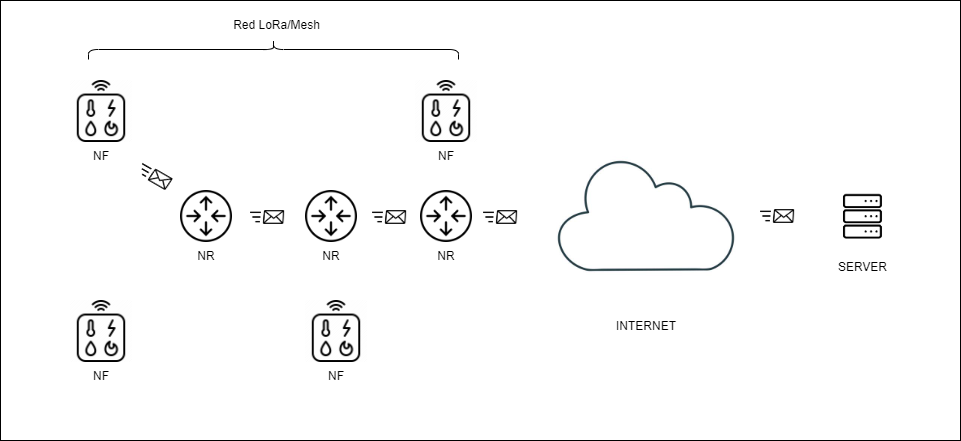
\includegraphics[width=1\textwidth]{./Figures/esquema_basico_de_red.drawio.png}
\caption{Esquema de red.}
\label{fig:Esquema de red}
\end{figure}
\chapter{Introducción específica} % Main chapter title

\label{Chapter2}

%----------------------------------------------------------------------------------------
%	SECTION 1
%----------------------------------------------------------------------------------------

En este capítulo se describen los escenarios posibles de aplicación, el módulo de hardware que se utilizó y extienden algunos conceptos mencionados previamente que serán útiles para comprender el trabajo realizado.

\section{Escenarios de posible aplicación}

Como fue mencionado en el capítulo anterior, este proyecto surge de la intención de extender los casos de uso para el “HRD-Radio-LoRa”. Los escenarios que se desean contemplar con aquellos donde no es posible por cuestiones técnicas y/o económicas desplegar la cantidad de \emph{gateways}  necesarios para brindar cobertura a toda la zona deseada. De ahí que la solución buscó utilizar una mecanismo basado en \emph{mesh} para así poder utilizar los equipos instalados como ruteadores de los mensajes de sus vecinos y así permitir extender la cobertura de la red.

Los escenarios en los cuales resulta más beneficiosos este desarrollo son en las industrias de Agro y el \emph{Oil\&Gas}. En ambos casos el acceso a la energía eléctrica y redes de telecomunicaciones no es factible en ciertas zonas, lo que imposibilita la instalación de \emph{gateways}. En el caso particular de la industria de \emph{Oil\&Gas} también la propia geografía de la zona tiene un impacto negativo en las comunicaciones presentando una dificultad adicional. 


\section{Componentes de hardware}

El módulo de hardware sobre el cuál se realizó el desarrollo fue el “HRD-Radio-LoRa”.~\ref{fig:Hardware} \citep{WEBSITE:5} Los componentes principales son un transceptor LoRa de marca HOPERF, un microcontrolador de 16 bits de marca Microchip y un \emph{bus} de datos que permite a la placa comunicarse con otros módulos también fabricados por RF Industrial.


\begin{figure}
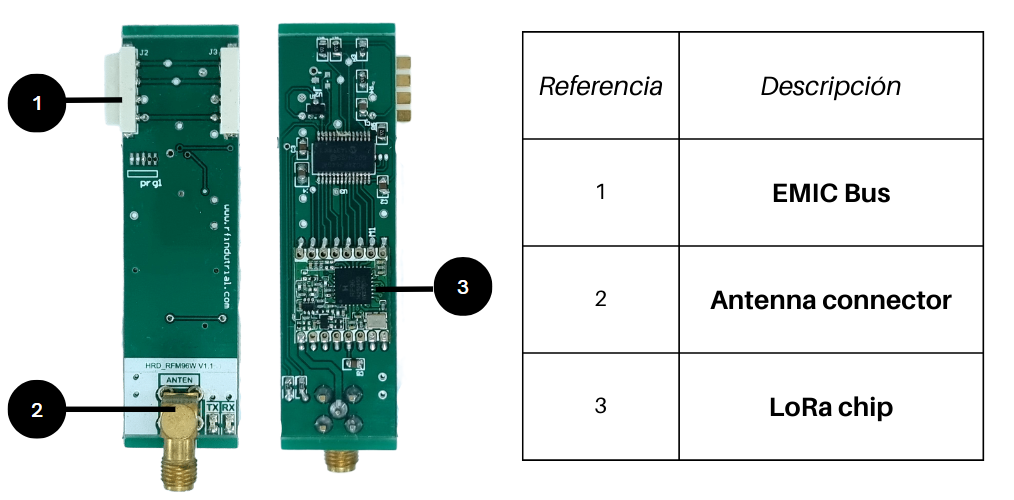
\includegraphics[width=1\textwidth]{./Figures/EMIC-radio-lora.png}
\caption{Esquema de red.}
\label{fig:Hardware}
\end{figure}

\section{Protocolo de enrutamiento}

Un protocolo de enrutamiento de paquetes es un conjunto de reglas y procedimientos que se utilizan para determinar cómo se transmiten los paquetes de datos a través de una red de dispositivos. Estos protocolos permiten que los paquetes sean enviados de manera eficiente desde el origen al destino a través de una serie de nodos intermedios.

El enrutamiento de paquetes implica tomar decisiones sobre la mejor ruta para enviar los paquetes en función de la topología y las condiciones actuales de la red. A continuación se mencionan algunos de las principales problemáticas a ser resueltas por un protocolo de enrutamiento.

\subsection{Descubrimiento de la topología}

El protocolo necesita conocer la estructura y los enlaces de la red para tomar decisiones de enrutamiento. Esto lo logra intercambiando estableciendo los mecanismos necesarios para que los nodos de la red puedan intercambiar información de estado o de enlace.

\subsection{Construcción de la tabla de enrutamiento}

Cada nodo de la red mantiene una tabla de enrutamiento que indica las rutas disponibles hacia diferentes destinos. Esta tabla se crea a partir de la información recopilada durante el descubrimiento de la topología y se actualiza dinámicamente a medida que la red cambia.

\subsection{Selección de la mejor ruta}

Basándose en la información de la tabla de enrutamiento, cada nodo toma decisiones sobre la ruta óptima para enviar los paquetes. Al momento de tomar estas decisiones se pueden considerar una sería de  métricas, como la latencia, el ancho de banda o el costo de los enlaces.

\subsection{Actualización de la información de enrutamiento}

Los protocolos de enrutamiento utilizan diferentes mecanismos para mantener la información de enrutamiento actualizada. Esto puede incluir la difusión periódica de actualizaciones de enrutamiento, el intercambio de mensajes de estado entre nodos adyacentes o la detección de cambios en la topología de la red.

\subsection{Resolución de problemas y enrutamiento alternativo}

Los protocolos de enrutamiento deben manejar situaciones en las que se producen fallas o congestión en los enlaces de la red. Esto implica detectar y resolver problemas de enrutamiento, así como encontrar rutas alternativas cuando una ruta principal no está disponible.

\section{Enrutamiento de vector distancia}

Cada router mantiene una tabla  que contiene información sobre las rutas disponibles y las distancias asociadas a cada destino. La distancia generalmente se mide en términos de saltos o en otras métricas como el costo, el retardo o el ancho de banda.\citep{rip}

\section{Requisitos de la implementación}

Como se ha mencionado anteriormente el proyecto surgió a partir de la necesidad de poder desplegar redes más robustas haciendo uso del módulo "HRD-Radio LoRa". Para esto se buscó desarrollar un protocolo que pudiese ser ejecutado sobre estos dispositivos y pudiera dotar a las redes de una serie de características que se describen en los siguientes párrafos.

Se deberá contemplar la existencia de tres tipos de elementos. Los servidores externos, los nodos finales y los nodos ruteadores.

Los servidores externos representan dispositivos que existen fuera de la red generada con los "HRD-Radio-LoRa". Su función es la de intercambiar datos con los nodos finales.

Los nodos finales son dispositivos que existen dentro de la red generada con los "HRD-Radio-LoRa". Son los encargados de generar los datos destinados a los servidores externos y también cuentan con la capacidad para recibir datos que estos envíen hacia ellos. La mayor parte del tiempo se mantienen en estado de bajo consumo, lo que implica que quedan fuera de la red. Sólo acceden a la red cuando necesitan enviar datos hacia los servidores externos. Una vez que envían esos datos, permanecen durante un tiempo esperando por datos que pudieran llegar de los servidores externos al cabo del cuál vuelven a pasar a estado de bajo consumo.

Los nodos ruteadores son dispositivos que existen dentro de la red generada con los "HRD-Radio-LoRa". Su función es la de trasladar los datos intercambiados entre los nodos finales y los servidores externos. Para esto intercambian con sus pares mensajes con información de ruteo de manera de lograr mantener la información de las rutas a cada destino actualizadas.



 
%\include{Chapters/Chapter3}
%\include{Chapters/Chapter4} 
%\include{Chapters/Chapter5} 

%----------------------------------------------------------------------------------------
%	CONTENIDO DE LA MEMORIA  - APÉNDICES
%----------------------------------------------------------------------------------------

\appendix % indicativo para indicarle a LaTeX los siguientes "capítulos" son apéndices

% Incluir los apéndices de la memoria como archivos separadas desde la carpeta Appendices
% Descomentar las líneas a medida que se escriben los apéndices

%\include{Appendices/AppendixA}
%\include{Appendices/AppendixB}
%\include{Appendices/AppendixC}

%----------------------------------------------------------------------------------------
%	BIBLIOGRAPHY
%----------------------------------------------------------------------------------------

\Urlmuskip=0mu plus 1mu\relax
\raggedright
\printbibliography[heading=bibintoc]

%----------------------------------------------------------------------------------------

\end{document}  
